Let $\tilde{\phi}(t)$ be a regular function, that estimates the spectral density.
Since $\phi(t)$ is no function in the classical sense, but all approximations are continuous functions,
\[
\left|\left|\phi(t) - \tilde{\phi}(t)\right|\right|_{L^p}
\]
is not defined, to estimate the error.
In the following, we will introduce two methods to circumvent this problem.
The first one uses the fact that $\delta(t)$ is a distribution that can be applied to test functions from the Schwartz space $\SR$,
while the second one regularizes $\delta$-functions by replacing them with continuous and smooth functions.
These two approaches are closely related, as we will see later.

\section{Resolution}
In practice, there is often no need to approximate all eigenvalues of $A$ exactly.
This would even be highly discontinuous, as we recall the intuitive approach with histograms.
The accuracy of the approximation should be oriented towards the desired \emph{resolution}.
This means that often only the eigenvalues in a certain subinterval $[a, b] \subset \sigma(A)$ are of interest in a certain context.
The size $b - a$ is then called the resolution of the estimate.
This insight should be taken as a parameter in our further considerations.

\section{Restriction on the Schwartz space}
In this first method, we consider $\delta(t)$ as a distribution.
Let $g \in \Cinfty(\R)$ be a test function from the Schwartz space $\SR$ defined in Definition \ref{def:Schwartz space}.
Then we have
\[
\langle \delta(\cdot - \lambda), g \rangle = \int\limits_{-\infty}^{\infty} \delta(t - \lambda) g(t) \dt = g(\lambda)
\]
and for all $p, k \in \N_0$
\[
\sup_{t \in \R} |t^pg^{(k)}(t)| < \infty
\]
The error can therefore be measured as follows:
\[
\epsilon_1 = \sup_{g \in \SR} \left| \langle \phi, g \rangle - \langle \tilde{\phi}, g \rangle \right|
\]

To transfer the concept of resolution to this error,
we first consider $\nu_{[a, b]}$ from equation \ref{eq:nu_a_b} and define accordingly
\[
\tilde{\nu}_{[a, b]} = \int\limits_a^b n \tilde{\phi}(t) \dt
\]
with $\tilde{\phi}(t) \in \Cinfty(\R)$.
Assuming $n = 1$ and thus $\phi(t) = \delta(t)$,
an infinite resolution would mean that for arbitrarily small intervals $[a, b]$ the term $\left| \nu_{[a, b]} - \tilde{\nu}_{[a, b]} \right|$ also becomes arbitrarily small.
Let $a = -\varepsilon, b = \varepsilon$.
From the definition of the $\delta$-function it follows that
$$\lim \limits_{\varepsilon \to 0+} \nu_{[-\varepsilon, \varepsilon]} = 1$$
while for smooth functions $\tilde{\phi}$ it is clear that
$$\lim \limits_{\varepsilon \to 0+} \tilde{\nu}_{[-\varepsilon, \varepsilon]} = 0$$
This shows that no smooth function converges to the spectral density under continuous increase of the resolution.
A carefully balanced approximation would therefore be as precise as a constant one.
However, as noted earlier,
a finite resolution is often sufficient.
We can therefore restrict the Schwartz space $\SR$.
For example, one could only consider Gaussian distributions of the form
$$g_{\sigma}(t) = \frac{1}{(2\pi\sigma^2)^\frac{1}{2}}e^{-\frac{t^2}{2\sigma^2}}$$
and restrict $\SR$ to the subspace
$$\SR(\sigma;[\lambda_{us}, \lambda_{os}]) = \left\{ g \mid g(t) \equiv g_{\sigma}(t - \lambda), \lambda \in [\lambda_{us}, \lambda_{os}] \right\}$$
Here, $\lambda_{us}$ and $\lambda_{os}$ are the upper and lower bounds of the eigenvalues of $A$ as in the previous section,
while the parameter $\sigma$ represents the \emph{target resolution}.
We can now use the following metric for quality assessment:

\begin{equation} \label{eq:error}
    E\left[\tilde{\phi};\SR\left(\sigma; \left[\lambda_{lb}, \lambda_{ub} \right] \right)\right] = \sup_{g \in \SR(\sigma;[\lambda_{lb}, \lambda_{ub}])} \left| \langle \phi, g \rangle - \langle \tilde{\phi}, g \rangle \right|
\end{equation}

\section{Regularizing the Dirac delta distribution}
In the second method, we regularize the $\delta$-function.
This means that we replace the $\delta$-function with a smooth function $\phi(t)$
that approximates the spectral density.
This is done by smoothing the $\delta$-function.
For example, we can use the Gaussian distribution with standard deviation $\sigma$:
$$\phi_{\sigma}(t) = \frac{1}{(2\pi\sigma^2)^\frac{1}{2}}e^{-\frac{t^2}{2\sigma^2}}$$
This function is smooth and well-defined for all $t \in \R$.
It is also normalized, meaning that
$$\int\limits_{-\infty}^{\infty} \phi_{\sigma}(t) \dt = 1$$
This means that $\phi_{\sigma}(t)$ can be interpreted as a probability density function.
The parameter $\sigma$ controls the width of the Gaussian distribution
and thus the resolution of the approximation.
This means that the smaller $\sigma$ is, the more precise the approximation is,
but also the more sensitive it is to noise in the data.
This is a common approach in numerical analysis to approximate distributions with smooth functions.
The function $\phi_{\sigma}(t)$ is then well-defined and can be used to calculate the error for $p=1, 2$ and $\infty$:
\[
\epsilon_2 = \left|\left| \phi_{\sigma}(t) - \tilde{\phi}(t) \right|\right|_p
\]

Let
\[
\phi_{\sigma}(t) = \left \langle \phi(\cdot), g_{\sigma}(\cdot - t)\right \rangle = \sum_{j = 1}^n g_{\sigma}(t - \lambda_j)
\]
This is the convolution of the spectral density with the Gaussian function $g_{\sigma}$.
In similar manner, let
\[
\tilde{\phi}_{\sigma}(t) = \langle \tilde{\phi}(\cdot), g_{\sigma}(\cdot - t) \rangle
\]
Then
\[
E\left[\tilde{\phi};\SR\left(\sigma; \left[\lambda_{lb}, \lambda_{ub} \right] \right)\right] = \sup_{g \in \SR(\sigma;[\lambda_{lb}, \lambda_{ub}])} \left| \phi_{\sigma}(t) - \tilde{\phi}_{\sigma}(t) \right|
\]
is the $L^\infty$ error between two well-defined functions.
Just like in the other method, $\sigma$ controls the resolution:
the larger the $\sigma$, the smoother but also less accurate the approximation.
For smaller values, one obtains coarser functions,
where small peaks can be detected exactly where the eigenvalues are located.
The following graphic is taken from \cite[p.~6]{linsaadyang14} and illustrates this effect for four different values of $\sigma$:
Sei also
$$\phi_{\sigma}(t) = \left \langle \phi(\cdot), g_{\sigma}(\cdot - t)\right \rangle = \sum_{j = 1}^n g_{\sigma}(t - \lambda_j)$$
Dies ist dann nicht anderes als die "Weichzeichnung" der Spektraldichte durch Gauß-Funktionen der Breite $\sigma$.

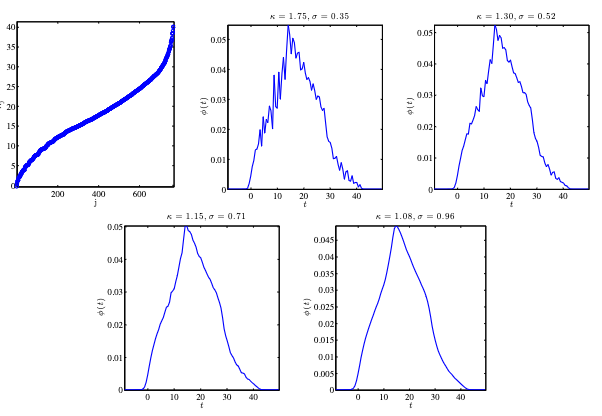
\includegraphics[height=7.5cm]{./Graphics/screenshot.png}

\section{The condition of non-negativity}
As a probability distribution, the spectral density is non-negative, meaning
\[
\forall g \in \SR, g \geq 0: \langle \phi, g \rangle \geq 0
\]
Some numerical approximations break this property, including the Kernel Polynomial Method.
This leads to large errors and must be considered carefully.
Methods to mitigate these negative effects would exceed the scope of this work.